\chapter{Introducción}
El presente Trabajo de Fin de Máster (TFM) se ocupa de afrontar una problemática real dentro del campo de la identificación humana \cite{thompson_forensic_2006}. En concreto, se hace uso de métodos de aprendizaje profundo y visión por computador para automatizar una técnica de antropología forense empleada en tareas de estimación del perfil biológico, más específicamente, la estimación de la edad de personas fallecidas a partir de restos óseos. 

Este capítulo introductorio se centra en presentar el problema en detalle, la motivación que nos lleva a enfrentarnos a él y el objetivo principal abordado en este TFM. 


\section{Definición del Problema}
\label{daIntro_ProblemDef}
%Que es la antropología forense
La antropología forense (AF) es la disciplina que se dedica al estudio y análisis detallado de las estructuras óseas del cuerpo humano con propósitos médico-legales \cite{byers_introduction_2016,RefWorks:RefID:17-christensen2019forensic}. Este campo combina conocimientos de la antropología física y de otras ramas afines para proporcionar información clave en investigaciones legales.

La antropología física, a su vez, es el campo que estudia la evolución de la especie humana, así como de las condiciones de vida y salud de distintas poblaciones, tanto antiguas como contemporáneas, mediante estudios osteológicos (del hueso) y somatológicos (del cuerpo) \cite{jurmain_introduction_2018}. Este conocimiento no solo permite un análisis detallado de los restos óseos, sino que también incluye una comprensión integral de los aspectos sociales, culturales y de comportamiento humano \cite{antrofisica}. Los expertos en AF, a través de este enfoque multidisciplinario, examinan minuciosamente los restos óseos para extraer la mayor cantidad posible de información relevante, la cual se utiliza para lograr los siguientes objetivos:

\begin{enumerate}
    \item Establecer la ascendencia y las características morfológicas del fallecido.
    \item Identificar las circunstancias y el modo en que ocurrió la muerte de la persona.
    \item Determinar el tiempo transcurrido desde el fallecimiento.
    \item Colaborar en la recuperación de restos, tanto superficiales como enterrados, que sean de interés para la investigación forense.
    \item Proporcionar información útil para la identificación de personas fallecidas, basándose en las características morfológicas presentes en los huesos humanos.
    \item Analizar el esqueleto de personas vivas con fines médico-legales, como en el caso de la identificación de migrantes o menores desaparecidos.
\end{enumerate}

La estimación del perfil biológico (PB) constituye una de las áreas fundamentales de la AF, e incluye la determinación de la edad, el sexo, la estatura y el origen poblacional o ascendencia, además de cualquier otra particularidad que ayude a individualizar los restos, ya sea total o parcialmente esqueletizados. La finalidad de esta evaluación es facilitar la búsqueda de la identidad de una persona desaparecida y, de ser posible, lograr una identificación positiva y certera. Un esquema ilustrativo del proceso de identificación forense puede apreciarse en la Figura \ref{fig:intro_1}.

\begin{figure}[h]
    \centering
    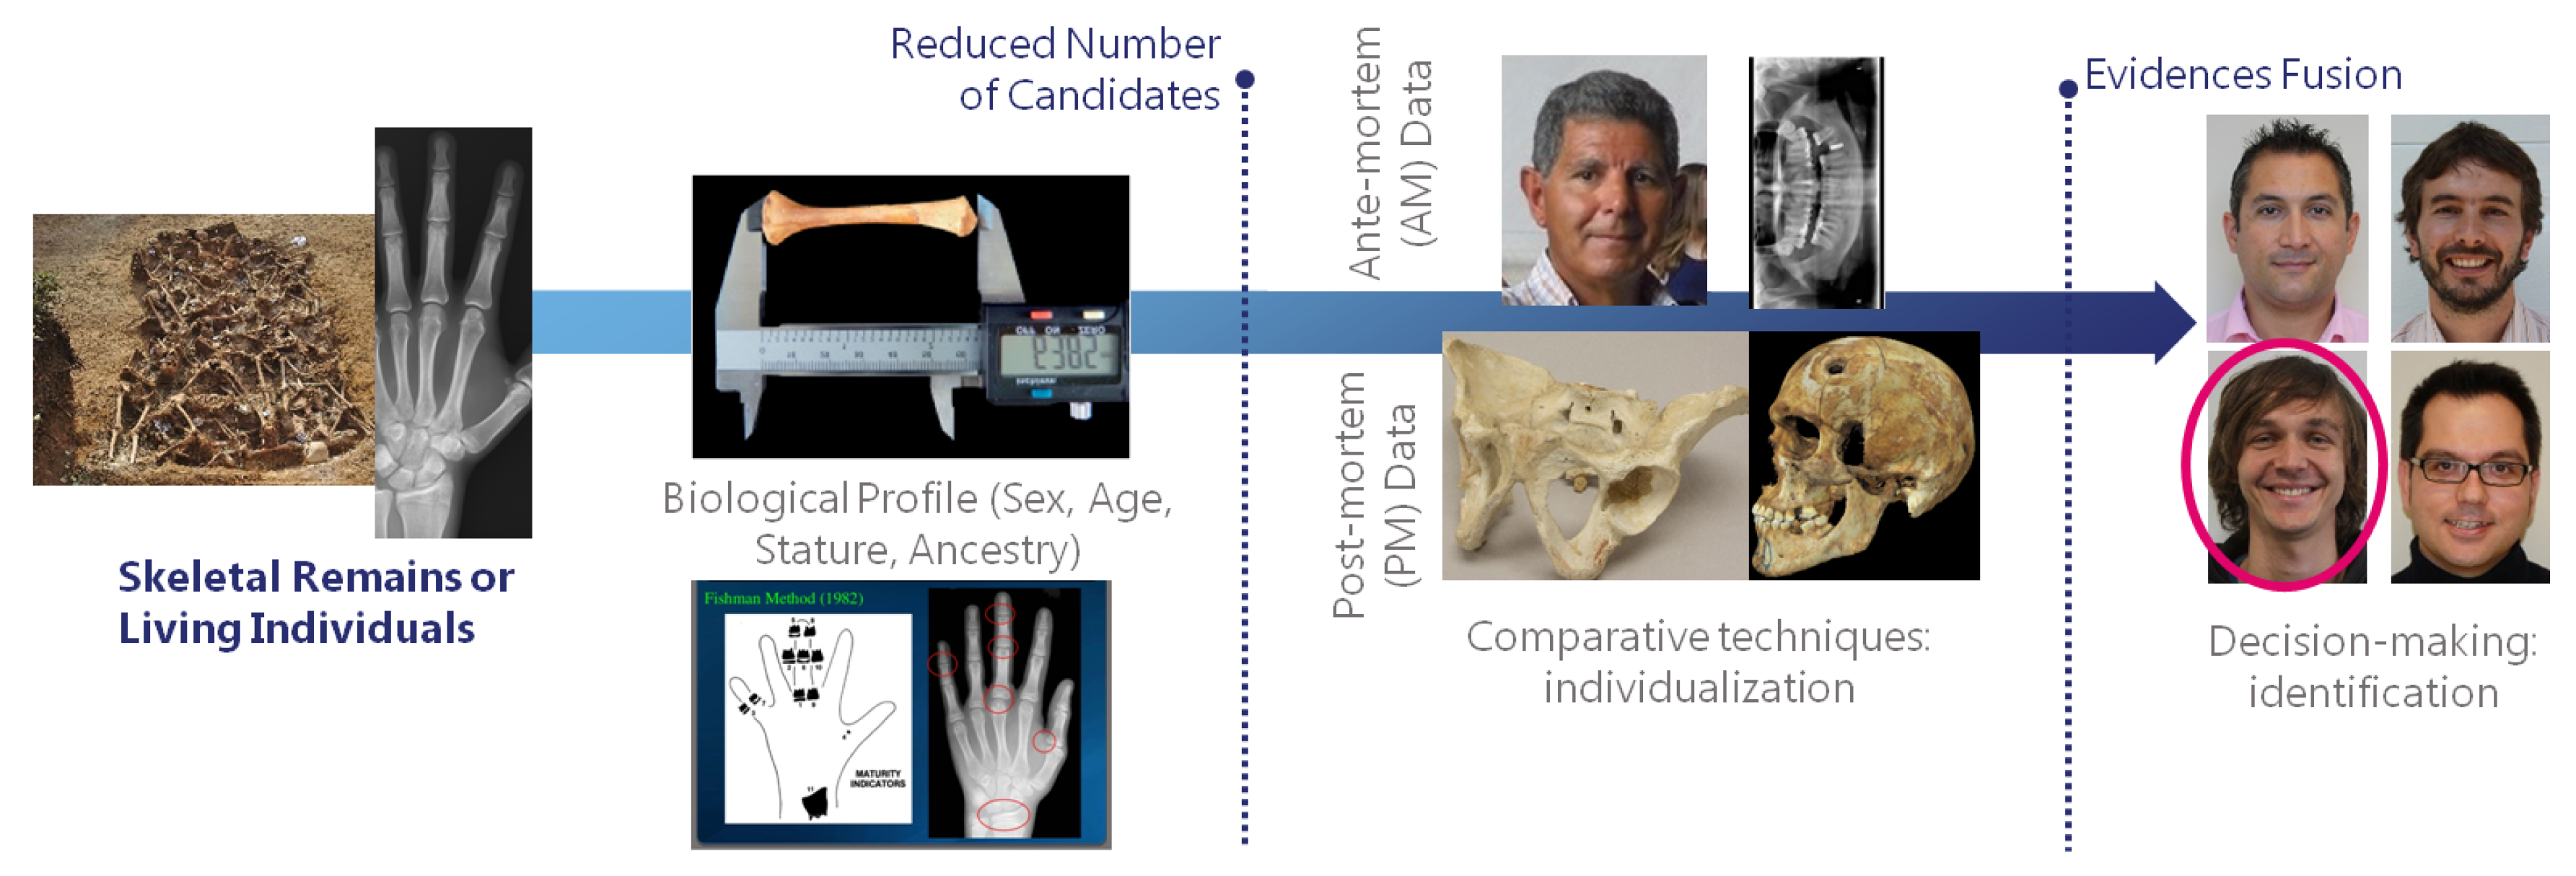
\includegraphics[width=1\linewidth]{figures/1_introduction/intro_1.png}
    \caption[Proceso general de identificación forense a partir de restos óseos o individuos vivos]{Proceso general de identificación forense a partir de restos óseos o individuos vivos mediante técnicas de análisis de imágenes biomédicas. A partir de los restos óseos o radiografías, se estima el perfil biológico (sexo, edad, estatura y ascendencia), lo cual permite reducir el número de posibles candidatos. Posteriormente, se realiza la comparación entre datos post-mortem y datos ante-mortem, utilizando técnicas comparativas como la superposición craneofacial o el análisis de estructuras dentales y esqueléticas. Finalmente, la fusión de evidencias conduce al proceso de toma de decisiones e identificación del individuo. Figura tomada de \cite{RefWorks:RefID:21-mesejo2020survey}.}
    \label{fig:intro_1}
\end{figure}

Uno de los aspectos fundamentales del PB es la estimación de la edad de los restos. Para lograrla, se examinan estructuras como las suturas craneales \cite{skullAF}, las costillas \cite{icscan1984age}, la cara auricular del ilion \cite{buckberry_age_2002} y la sínfisis del pubis \cite{garvin_current_2012}, estos dos últimos localizados en la pelvis. En cada caso, se observa el grado de desgaste que presentan estos huesos en el momento del fallecimiento, lo cual permite aproximarse a la edad del individuo \cite{RefWorks:RefID:12-black2011forensic}.

La sínfisis del pubis es el hueso más utilizado para estimar la edad de un individuo ya fallecido, siendo la opción preferida por el 95\% de los antropólogos forenses \cite{garvin_current_2012}. El método predominante se fundamenta en el trabajo pionero de Thomas Wingate Todd \cite{RefWorks:RefID:19-todd1921age}, quien en 1921 documentó las transformaciones progresivas de la sínfisis del pubis con el envejecimiento, permitiendo estimar un rango aproximado de edad al momento del fallecimiento. Todd propuso un sistema de etapas de envejecimiento que ha sido revisado y perfeccionado en múltiples ocasiones, siendo la revisión de Suchey-Brooks \cite{RefWorks:RefID:20-brooks1990skeletal}, publicada en 1990, posiblemente la más reconocida de todas. Tanto el método original de Todd como la revisión de Suchey-Brooks se basan en el análisis de diferentes características de la sínfisis del pubis. En función del estado de cada una, asignan atributos categóricos que reflejan el grado de erosión ósea en distintas áreas, permitiendo así calcular un rango estimado de edad para el difunto. Dichas características varían según el método, en este TFM se utilizan las 9 características propuestas por Villar et al. \cite{villar2017first} y descritas en un atlas propuesto por \cite{irurita2025pubic} para el método de Todd, que se detallan en la Tabla \ref{table:themBones}, y en la Tabla \ref{themBomes:visualExample} se presenta un ejemplo visual de algunas.

\begin{table}[h]
    \centering
% \resizebox{\textwidth}{!}{%
\begin{tabular}{ccc}
    \hline
    \rowcolor[HTML]{D33333} 
    \multicolumn{1}{c|}{\cellcolor[HTML]{D33333}{\color[HTML]{FFFFFF} Característica}} & \multicolumn{2}{c}{\cellcolor[HTML]{D33333}{\color[HTML]{FFFFFF} Atributos}} \\ \hline
    \rowcolor[HTML]{FFCCC9} 
    \multicolumn{1}{|c}{\cellcolor[HTML]{FD6864}Crestas y Surcos} & Porosidad Regular & \multicolumn{1}{c|}{\cellcolor[HTML]{FFCCC9}Muy Definidas} \\ \cline{1-1}
    \multicolumn{1}{c|}{} & \cellcolor[HTML]{FFCCC9}Poco Profundas & \multicolumn{1}{c|}{\cellcolor[HTML]{FFCCC9}Restos de Surcos} \\ \cline{3-3} 
    \multicolumn{1}{c|}{} & \multicolumn{1}{c|}{\cellcolor[HTML]{FFCCC9}No hay surcos} &  \\ \hline
    \rowcolor[HTML]{FFCCC9} 
    \multicolumn{1}{|c}{\cellcolor[HTML]{FD6864}Porosidad Irregular} & No & \multicolumn{1}{c|}{\cellcolor[HTML]{FFCCC9}Mediana} \\ \cline{1-1} \cline{3-3} 
    \multicolumn{1}{c|}{} & \multicolumn{1}{c|}{\cellcolor[HTML]{FFCCC9}Si} &  \\ \hline
    \rowcolor[HTML]{FFCCC9} 
    \multicolumn{1}{|c}{\cellcolor[HTML]{FD6864}Borde Superior} & No Definido & \multicolumn{1}{c|}{\cellcolor[HTML]{FFCCC9}Definido} \\ \hline
    \rowcolor[HTML]{FFCCC9} 
    \multicolumn{1}{|c}{\cellcolor[HTML]{FD6864}Nódulo Óseo} & Ausente & \multicolumn{1}{c|}{\cellcolor[HTML]{FFCCC9}Presente} \\ \hline
    \rowcolor[HTML]{FFCCC9} 
    \multicolumn{1}{|c}{\cellcolor[HTML]{FD6864}Borde Inferior} & No Definido & \multicolumn{1}{c|}{\cellcolor[HTML]{FFCCC9}Definido} \\ \hline
    \rowcolor[HTML]{FFCCC9} 
    \multicolumn{1}{|c}{\cellcolor[HTML]{FD6864}Plataforma Dorsal} & Ausente & \multicolumn{1}{c|}{\cellcolor[HTML]{FFCCC9}En Formación} \\ \cline{1-1} \cline{3-3} 
    \multicolumn{1}{l|}{} & \multicolumn{1}{c|}{\cellcolor[HTML]{FFCCC9}Presente} & \multicolumn{1}{l}{} \\ \hline
    \rowcolor[HTML]{FFCCC9} 
    \multicolumn{1}{|c}{\cellcolor[HTML]{FD6864}Borde Dorsal} & Ausente & \multicolumn{1}{c|}{\cellcolor[HTML]{FFCCC9}En Formación} \\ \cline{1-1} \cline{3-3} 
    \multicolumn{1}{l|}{} & \multicolumn{1}{c|}{\cellcolor[HTML]{FFCCC9}Presente} & \multicolumn{1}{l}{} \\ \hline
    \rowcolor[HTML]{FFCCC9} 
    \multicolumn{1}{|c}{\cellcolor[HTML]{FD6864}Bisel Ventral} & Ausente & \multicolumn{1}{c|}{\cellcolor[HTML]{FFCCC9}En Formación} \\ \cline{1-1} \cline{3-3} 
    \multicolumn{1}{c|}{} & \multicolumn{1}{c|}{\cellcolor[HTML]{FFCCC9}Presente} &  \\ \hline
    \rowcolor[HTML]{FFCCC9} 
    \multicolumn{1}{|c}{\cellcolor[HTML]{FD6864}Borde Ventral} & Ausente & \multicolumn{1}{c|}{\cellcolor[HTML]{FFCCC9}En Formación} \\ \cline{1-1}
    \multicolumn{1}{c|}{} & \cellcolor[HTML]{FFCCC9}Formado, Sin Excrecencias & \multicolumn{1}{c|}{\cellcolor[HTML]{FFCCC9}Formado, Pocas Excrecencias} \\ \cline{3-3} 
    \multicolumn{1}{c|}{} & \multicolumn{1}{c|}{\cellcolor[HTML]{FFCCC9}Formado, Muchas Excrecencias} &  \\ \cline{2-2}
\end{tabular}%
% }
\caption[Método de Todd: Características y atributos para determinación de edad]{Características y atributos utilizados para la determinación de la edad según el método de Todd \cite{RefWorks:RefID:19-todd1921age} propuestos en Villar et al. \cite{villar2017first}.}
\label{table:themBones}
\end{table}

\begin{table}[htbp]
    \centering
    \begin{tabular}{|
    >{\columncolor[HTML]{D33333}}c |c|cc}
    \hline
    {\color[HTML]{FFFFFF} \textbf{Característica}} & \begin{tabular}[c]{@{}c@{}}Crestas y Surcos\end{tabular} & \multicolumn{1}{c|}{\begin{tabular}[c]{@{}c@{}}Porosidad  Irregular\end{tabular}} & \multicolumn{1}{c|}{\begin{tabular}[c]{@{}c@{}}Borde Superior\end{tabular}} \\ \hline
    {\color[HTML]{FFFFFF} \textbf{Atributo}} & Muy Definidos & \multicolumn{1}{c|}{Sí} & \multicolumn{1}{c|}{Definido} \\ \hline
    {\color[HTML]{FFFFFF} \textbf{Ejemplo}} & 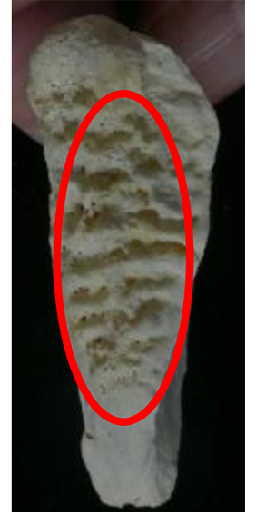
\includegraphics[align=c, width=0.2\linewidth]{figures/1_introduction/todd1.png} & \multicolumn{1}{c|}{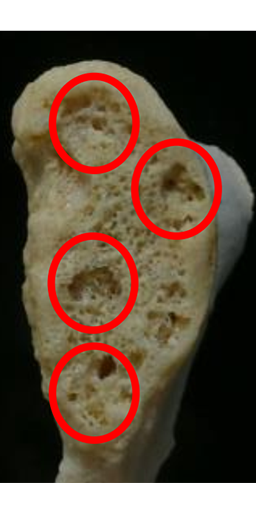
\includegraphics[align=c, width=0.2\linewidth]{figures/1_introduction/todd2.png}} & \multicolumn{1}{c|}{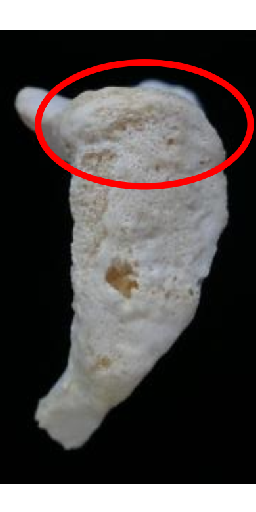
\includegraphics[align=c, width=0.2\linewidth]{figures/1_introduction/todd3.png}} \\ \hline
    {\color[HTML]{FFFFFF} \textbf{Característica}} & \begin{tabular}[c]{@{}c@{}}Nódulo Óseo\end{tabular} & \multicolumn{1}{c|}{\begin{tabular}[c]{@{}c@{}}Borde Inferior\end{tabular}} & \multicolumn{1}{c|}{\begin{tabular}[c]{@{}c@{}}Borde Dorsal\end{tabular}} \\ \hline
    {\color[HTML]{FFFFFF} \textbf{Atributo}} & Presente & \multicolumn{1}{c|}{Definido} & \multicolumn{1}{c|}{Definido} \\ \hline
    {\color[HTML]{FFFFFF} \textbf{Ejemplo}} & 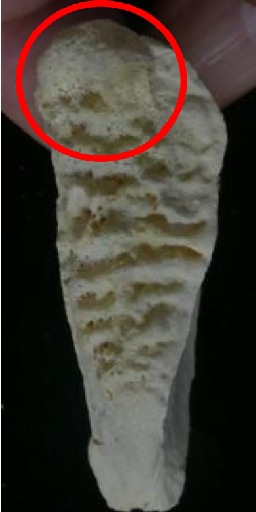
\includegraphics[align=c, width=0.2\linewidth]{figures/1_introduction/todd4.png} & \multicolumn{1}{c|}{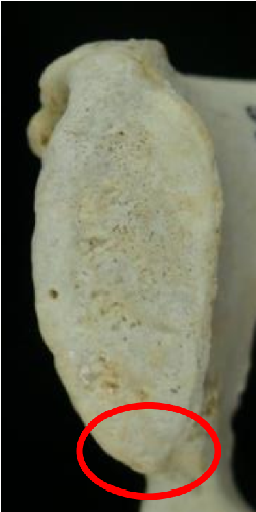
\includegraphics[align=c, width=0.2\linewidth]{figures/1_introduction/todd5.png}} & \multicolumn{1}{c|}{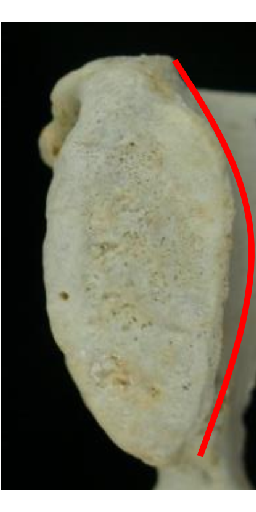
\includegraphics[align=c, width=0.2\linewidth]{figures/1_introduction/todd6.png}} \\ \hline
    {\color[HTML]{FFFFFF} \textbf{Característica}} & \begin{tabular}[c]{@{}c@{}}Plataforma Dorsal\end{tabular} & \multicolumn{1}{l}{} & \multicolumn{1}{l}{} \\ \cline{1-2}
    {\color[HTML]{FFFFFF} \textbf{Atributo}} & Presente & \multicolumn{1}{l}{} & \multicolumn{1}{l}{} \\ \cline{1-2}
    {\color[HTML]{FFFFFF} \textbf{Ejemplo}} & 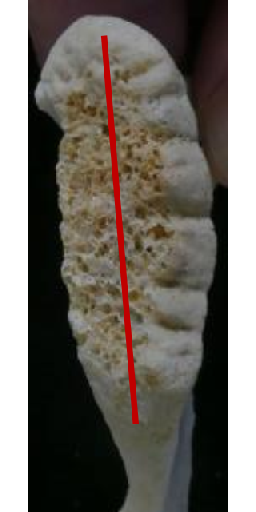
\includegraphics[align=c, width=0.2\linewidth]{figures/1_introduction/todd7.png} & \multicolumn{1}{l}{} & \multicolumn{1}{l}{} \\ \cline{1-2}
    \end{tabular}
    \caption[Método de Todd: Ejemplo visual de algunas características y atributos]{Ejemplos visuales de algunas de las características y atributos del método de Todd.}
    \label{themBomes:visualExample}
\end{table}

Es importante destacar que, al igual que en muchas otras tareas de la AF, la anotación de las características en las que se basan los métodos de estimación de la edad señalados depende en gran medida del criterio subjetivo del experto. Esto genera errores intra- e inter-experto \cite{irurita2025pubic}, ya que el uso de criterios subjetivos y descriptivos introduce limitaciones debido a las diversas interpretaciones entre evaluadores \cite{RefWorks:RefID:12-black2011forensic}. Tal situación disminuye la confiabilidad y validez de los resultados obtenidos, lo que finalmente reduce la credibilidad de los estudios forenses cuando se presentan como evidencia en un juicio (como se indicará más abajo cuando se mencione el estándar de Daubert). Esta problemática justifica la búsqueda de herramientas y metodologías que, al menos parcialmente, mitiguen dichas limitaciones. En este contexto, disciplinas como la inteligencia artificial (IA) \cite{russell_artificial_2021} y, en particular, el aprendizaje automático (\textit{Machine Learning}, ML) \cite{abu-mostafa_learning_2012, bishop_pattern_2019, murphy_probabilistic_2022, murphy_probabilistic_2023}, el aprendizaje profundo (\textit{Deep Learning}, DL) \cite{Goodfellow-et-al-2016, bishop_deep_2024, prince_understanding_2023} y la visión por computador (\textit{Computer Vision}, CV) \cite{torralba_foundations_2024, szeliski_computer_2022} pueden asistir, automatizar y acelerar las tareas forenses, reduciendo significativamente los sesgos y errores.

Considerando todo lo anterior, \textbf{el presente TFM se centra en la clasificación automática de las características morfológicas de la sínfisis del pubis para estimar la edad de la muerte a partir de modelos 3D mediante técnicas de IA.}

\section{Motivación}
En las últimas décadas los avances en IA, especialmente en ML y CV, han facilitado tanto la automatización de tareas repetitivas y tediosas como la superación del rendimiento humano en actividades complejas. En estos ámbitos, se han logrado avances significativos en tareas como la clasificación y segmentación de imágenes \cite{edozie_comprehensive_2025}, la detección de objetos en las mismas \cite{liu_deep_2020}, generación de imagen y vídeo \cite{wang_generative_2021} así como la reconstrucción de imágenes \cite{xie_review_2022}. Estas técnicas han sido ampliamente adoptadas en diversas disciplinas \cite{chai_deep_2021}, incluida la medicina, donde han proporcionado herramientas de gran utilidad para los profesionales del área \cite{esteva_deep_2021}.

No obstante, resulta sorprendente que, en la actualidad, la AF siga presentando un nivel relativamente bajo de sofisticación tecnológica \cite{RefWorks:RefID:21-mesejo2020survey}. En este contexto, una de las principales motivaciones de este trabajo es impulsar la modernización y automatización de la AF desde una perspectiva tecnológica, centrándose particularmente en la aplicación de técnicas avanzadas para la estimación de edad.

Además, como se mencionó previamente, la subjetividad inherente a la AF representa un desafío desde el punto de vista legal. En muchos casos, los análisis carecen de una base científica sólida según el criterio de Daubert \cite{noauthor_daubert_nodate}, el cual establece los requisitos para la admisibilidad del testimonio experto en un juicio. Según este criterio, un método es válido si: (1) los resultados son reproducibles y han sido verificados por terceros, (2) posee tasas de error conocidas y (3) es aceptado por la comunidad científica forense.

En este sentido, la aplicación de IA en AF puede contribuir significativamente a la reducción de la subjetividad en las identificaciones, minimizando errores humanos, y acelerando la realización de múltiples tareas, estructurando el conocimiento experto y facilitando la obtención de nuevos hallazgos. Esto, a su vez, fortalecería la base científica de los métodos utilizados en la disciplina, permitiendo que sean reproducibles y que se conozcan con precisión sus tasas de error, lo que favorecería su cumplimiento con el criterio de Daubert y su aceptación en el ámbito legal.

Si se analiza el contexto global de la identificación humana, se evidencia que la estimación del PB mediante técnicas de AF adquiere especial relevancia, puesto que otras herramientas de mayor precisión y sofisticación, como el análisis de ADN o la toma de huellas dactilares, presentan limitaciones significativas \cite{de_boer_role_2019, beauthier_mass_2009}. Por ejemplo, el análisis de ADN requiere una inversión elevada en recursos y tiempo, y al igual que la obtención de huellas dactilares, depende de la disponibilidad de datos tanto ante-mortem como post-mortem. Además, ambas técnicas se ven afectadas por el estado de los tejidos blandos, que son los más susceptibles a la descomposición natural o a daños provocados por quemaduras y exposición a agua o productos químicos, entre otros factores. En cambio, el tejido óseo, en general, demuestra una mayor resistencia y es frecuentemente lo único recuperable tras la completa descomposición de los tejidos blandos. Por ello, las técnicas basadas en AF son especialmente útiles en los siguientes escenarios:

\begin{itemize}
    \item Identificación masiva de víctimas de desastres naturales, accidentes o ataques terroristas.
    \item Identificación de víctimas de conflictos armados o actos de lesa humanidad, donde los restos pueden estar desmembrados, desfigurados y/o quemados.
    \item Procesamiento de fosas comunes en las que los restos óseos se han mezclado.
    \item Identificación de personas desaparecidas en contextos no relacionados con desastres o guerras, en los que las condiciones del cadáver han impedido la aplicación de otras técnicas \cite{byers_introduction_2016}.
\end{itemize}

Para dimensionar el desafío al que se enfrentan los antropólogos forenses, es relevante considerar que, únicamente en el año 2019, 20,000 personas perdieron la vida por causas vinculadas al terrorismo, con un promedio anual de 24,000 muertes en la última década atribuibles a este fenómeno \cite{owid_terrorism}. Asimismo, los desastres naturales ocasionan aproximadamente entre 40,000 y 50,000 muertes anuales \cite{owid_natural_disasters}. En el caso de Gaza, al momento de la redacción de este documento, se estima que entre 56,000 y 80,000 personas han sido asesinadas como resultado de los bombardeos, mientras que al menos 11.000 permanecen desaparecidas bajo los escombros, según datos del Ministerio de Salud y la ONU \cite{morales_56000_2025}. En España, aún se deben recuperar alrededor de 20,000 víctimas de la Guerra Civil, muchas de las cuales se hallan en fosas y cunetas, de modo que apenas un tercio de ellas podría ser identificada mediante análisis de ADN \cite{junquera_huellas_2022}.

Estos datos subrayan la necesidad de incorporar técnicas informáticas automatizadas en el ámbito de la AF, ya que permitirían una considerable optimización en términos de tiempo y recursos, facilitando la detección de las características determinantes para la estimación de la edad en situaciones en las que el número de individuos a identificar es elevado y otras técnicas no son aplicables.

\section{Objetivos}

Tras haber descrito el problema y su motivación, el objetivo principal de este TFM consiste en desarrollar y validar un modelo de aprendizaje profundo que, a partir de modelos 3D de la sínfisis púbica, permita extraer características morfológicas relevantes para la estimación de la edad en el momento de la muerte.

Cabe destacar que este trabajo se construye como una continuación directa del TFG desarrollado previamente por el propio autor \cite{lugli_tfg_2022}\footnote{Galardonado con el Premio a Mejor TFG del Grado de Ingeniería Informática por la E.T.S. de Ingenierías Informática y de Telecomunicación de la Universidad de Granada, 10 de mayo de 2023.}. En dicho trabajo preliminar se exploró un método que fue en ese momento el estado del arte para el procesamiento de los escaneos 3D de la sínfisis del pubis, donde solo se centró en la predicción de una de las nueve características morfológicas del método de Todd, concretamente el Nódulo Óseo. Se realizó con una cantidad mucho más restringida de datos y de capacidad de cómputo. Aun así se lograron resultados prometedores, siendo esta la razón de ser de este proyecto actual.

El presente TFM amplía sustancialmente dicho enfoque inicial, incorporando técnicas más actuales y sofisticadas de DL para datos 3D, así como procedimientos más avanzados para la obtención de la arquitectura e hiperparámetros de dichos modelos. Además, se aborda un volumen experimental considerablemente mayor y se incorpora el análisis del efecto de la resolución de las mallas sobre el rendimiento predictivo así como una visión a la interpretabilidad de los modelos obtenidos. Todo ello con el objetivo de avanzar hacia un sistema más robusto, reproducible y explicable para la clasificación automática de las características morfológicas utilizadas en la estimación de la edad de la muerte.

Este objetivo principal se desglosa en los siguientes objetivos parciales:

\begin{enumerate}
    \item Realizar un estudio exhaustivo de la literatura relativa a la estimación de edad a partir de restos óseos y al procesamiento de modelos 3D mediante redes neuronales profundas.
    \item Analizar y discutir los enfoques y modelos existentes, seleccionando de forma razonada los candidatos más prometedores para el problema abordado.
    \item Generar, entrenar y evaluar de forma extensiva múltiples arquitecturas de DL con el fin de identificar configuraciones óptimas que permitan predecir con precisión las nueve características morfológicas del método de Todd, tanto desde una perspectiva multiclase como multietiqueta.
\end{enumerate}

\section{Planificación del proyecto}

El presente trabajo consiste, en esencia, en el diseño e implementación de un software de carácter investigador. Para su planificación, es importante considerar que la asignatura del TFM está dotada con 12 créditos ECTS, lo que equivale a un total de 300 horas de trabajo, tomando como referencia que un crédito representa 25 horas.

Teniendo en cuenta que el autor compagina este proyecto con una actividad laboral a tiempo completo, se ha optado por una estimación conservadora que contempla la realización del TFM a lo largo de un curso académico completo, es decir, en un plazo aproximado de 40 semanas. Esto se traduce en una dedicación semanal de 7.5 horas, repartidas en sesiones de una hora y media diaria durante cinco días a la semana.

Dado que el proyecto cuenta con unos requisitos y objetivos bien definidos, no se prevén grandes desviaciones respecto a su desarrollo original. Por ello, se ha optado por emplear la metodología de desarrollo de software en cascada \cite{pressman2005software}, que organiza el proceso en fases secuenciales: análisis, diseño, codificación o desarrollo, pruebas y mantenimiento.

No obstante, es importante señalar que el modelo en cascada rara vez se aplica de forma estricta, ya que su estructura lineal impide retroceder a fases previas una vez completadas. Esto requeriría un conocimiento absoluto y estable de los requisitos desde el inicio, así como la ausencia de errores en etapas posteriores, condiciones poco realistas en la mayoría de proyectos de investigación. Por esta razón, se adopta una variante más flexible conocida como modelo en cascada con retroalimentación, que permite retornar a fases anteriores cuando sea necesario, ya sea para corregir errores, resolver ambigüedades o adaptar el diseño a cambios en los requisitos detectados durante el desarrollo.

Las fases del ciclo de vida del software se adaptaron al proyecto de la siguiente manera:

\begin{itemize}
\item \textbf{Análisis de Requisitos:} Esta fase incluyó las reuniones iniciales con los directores del TFM y los expertos en AF, quienes actuaron como usuarios finales del sistema. También se realizó una revisión bibliográfica exhaustiva, tanto en el ámbito de la AF como en su intersección con técnicas automáticas de inteligencia artificial. El objetivo fue establecer con precisión los objetivos del proyecto y delimitar su alcance.

\item \textbf{Diseño:} En esta etapa se investigaron y seleccionaron las técnicas más adecuadas para abordar el problema, incluyendo la elección de modelos, métricas y protocolos de validación experimental. Asimismo, se llevaron a cabo pruebas preliminares para verificar la viabilidad técnica de las distintas configuraciones y metodologías seleccionadas.

\item \textbf{Desarrollo:} Consistió en la adaptación del código base de las técnicas seleccionadas, así como en el desarrollo de funcionalidades adicionales. Se implementaron también herramientas de soporte en forma de \textit{scripts} para el preprocesado de los datos, así como para el cálculo automatizado de métricas y datos.

\item \textbf{Pruebas:} Esta fase se centró en la realización de experimentos sistemáticos sobre los modelos y configuraciones seleccionadas, con el objetivo de evaluar el rendimiento y extraer conclusiones sobre la efectividad de las soluciones propuestas.

\item \textbf{Informe:} En esta fase se procedió a la documentación de todo el proceso en el presente informe, detallando las motivaciones, fundamentos teóricos, metodología, resultados obtenidos, análisis y conclusiones del trabajo.
\end{itemize}

La planificación inicial del proyecto puede consultarse en la Tabla \ref{table:plan1}, en la cual se contempló un mes adicional como margen para posibles imprevistos o retrasos en la ejecución del trabajo. Se estimó un total de 307.5 horas totales para realizar el TFM.

\begin{table}[h]
\centering
\resizebox{\textwidth}{!}{%
\begin{tabular}{|c|c|ccccccccccccccccccccccc}
    \hline
    \rowcolor[HTML]{D33333} 
    \cellcolor[HTML]{D33333}{\color[HTML]{FFFFFF} } & \cellcolor[HTML]{D33333}{\color[HTML]{FFFFFF} } & \multicolumn{2}{c|}{\cellcolor[HTML]{D33333}{\color[HTML]{FFFFFF} \textbf{Septiembre}}} & \multicolumn{4}{c|}{\cellcolor[HTML]{D33333}{\color[HTML]{FFFFFF} \textbf{Octubre}}} & \multicolumn{4}{c|}{\cellcolor[HTML]{D33333}{\color[HTML]{FFFFFF} \textbf{Noviembre}}} & \multicolumn{5}{c|}{\cellcolor[HTML]{D33333}{\color[HTML]{FFFFFF} \textbf{Diciembre}}} & \multicolumn{4}{c|}{\cellcolor[HTML]{D33333}{\color[HTML]{FFFFFF} \textbf{Enero}}} & \multicolumn{4}{c|}{\cellcolor[HTML]{D33333}{\color[HTML]{FFFFFF} \textbf{Febrero}}} \\ \cline{3-25} 
    \rowcolor[HTML]{D33333} 
    \multirow{-2}{*}{\cellcolor[HTML]{D33333}{\color[HTML]{FFFFFF} \textbf{Tarea}}} & \multirow{-2}{*}{\cellcolor[HTML]{D33333}{\color[HTML]{FFFFFF} \textbf{\begin{tabular}[c]{@{}c@{}}Semanas – \\ Horas\end{tabular}}}} & \multicolumn{1}{c|}{\cellcolor[HTML]{D33333}{\color[HTML]{FFFFFF} \textbf{23}}} & \multicolumn{1}{c|}{\cellcolor[HTML]{D33333}{\color[HTML]{FFFFFF} \textbf{30}}} & \multicolumn{1}{c|}{\cellcolor[HTML]{D33333}{\color[HTML]{FFFFFF} \textbf{7}}} & \multicolumn{1}{c|}{\cellcolor[HTML]{D33333}{\color[HTML]{FFFFFF} \textbf{14}}} & \multicolumn{1}{c|}{\cellcolor[HTML]{D33333}{\color[HTML]{FFFFFF} \textbf{21}}} & \multicolumn{1}{c|}{\cellcolor[HTML]{D33333}{\color[HTML]{FFFFFF} \textbf{28}}} & \multicolumn{1}{c|}{\cellcolor[HTML]{D33333}{\color[HTML]{FFFFFF} \textbf{4}}} & \multicolumn{1}{c|}{\cellcolor[HTML]{D33333}{\color[HTML]{FFFFFF} \textbf{11}}} & \multicolumn{1}{c|}{\cellcolor[HTML]{D33333}{\color[HTML]{FFFFFF} \textbf{18}}} & \multicolumn{1}{c|}{\cellcolor[HTML]{D33333}{\color[HTML]{FFFFFF} \textbf{25}}} & \multicolumn{1}{c|}{\cellcolor[HTML]{D33333}{\color[HTML]{FFFFFF} \textbf{2}}} & \multicolumn{1}{c|}{\cellcolor[HTML]{D33333}{\color[HTML]{FFFFFF} \textbf{9}}} & \multicolumn{1}{c|}{\cellcolor[HTML]{D33333}{\color[HTML]{FFFFFF} \textbf{16}}} & \multicolumn{1}{c|}{\cellcolor[HTML]{D33333}{\color[HTML]{FFFFFF} \textbf{23}}} & \multicolumn{1}{c|}{\cellcolor[HTML]{D33333}{\color[HTML]{FFFFFF} \textbf{30}}} & \multicolumn{1}{c|}{\cellcolor[HTML]{D33333}{\color[HTML]{FFFFFF} \textbf{6}}} & \multicolumn{1}{c|}{\cellcolor[HTML]{D33333}{\color[HTML]{FFFFFF} \textbf{13}}} & \multicolumn{1}{c|}{\cellcolor[HTML]{D33333}{\color[HTML]{FFFFFF} \textbf{20}}} & \multicolumn{1}{c|}{\cellcolor[HTML]{D33333}{\color[HTML]{FFFFFF} \textbf{27}}} & \multicolumn{1}{c|}{\cellcolor[HTML]{D33333}{\color[HTML]{FFFFFF} \textbf{3}}} & \multicolumn{1}{c|}{\cellcolor[HTML]{D33333}{\color[HTML]{FFFFFF} \textbf{10}}} & \multicolumn{1}{c|}{\cellcolor[HTML]{D33333}{\color[HTML]{FFFFFF} \textbf{17}}} & \multicolumn{1}{c|}{\cellcolor[HTML]{D33333}{\color[HTML]{FFFFFF} \textbf{24}}} \\ \hline
    \textbf{\begin{tabular}[c]{@{}c@{}}Análisis \\ de Requisitos\end{tabular}} & 7 - 52.5 & \cellcolor[HTML]{FFCCC9} & \cellcolor[HTML]{FFCCC9} & \cellcolor[HTML]{FFCCC9} & \cellcolor[HTML]{FFCCC9} & \cellcolor[HTML]{FFCCC9} & \cellcolor[HTML]{FFCCC9} & \cellcolor[HTML]{FFCCC9} &  &  &  &  &  &  &  &  &  &  &  &  &  &  &  & \multicolumn{1}{c|}{} \\ \hline
    \textbf{Diseño} & 11 - 82.5 &  &  &  &  &  &  &  & \cellcolor[HTML]{FFCCC9} & \cellcolor[HTML]{FFCCC9} & \cellcolor[HTML]{FFCCC9} & \cellcolor[HTML]{FFCCC9} & \cellcolor[HTML]{FFCCC9} & \cellcolor[HTML]{FFCCC9} & \cellcolor[HTML]{FFCCC9} & \cellcolor[HTML]{FFCCC9} & \cellcolor[HTML]{FFCCC9} & \cellcolor[HTML]{FFCCC9} & \cellcolor[HTML]{FFCCC9} &  &  &  &  & \multicolumn{1}{c|}{} \\ \hline
    \textbf{Desarrollo} & 5 - 37.5 &  &  &  &  &  &  &  &  &  &  &  &  &  &  &  &  &  &  & \cellcolor[HTML]{FFCCC9} & \cellcolor[HTML]{FFCCC9} & \cellcolor[HTML]{FFCCC9} & \cellcolor[HTML]{FFCCC9} & \multicolumn{1}{c|}{\cellcolor[HTML]{FFCCC9}} \\ \hline
    \textbf{Pruebas} & 0 - 0 &  &  &  &  &  &  &  &  &  &  &  &  &  &  &  &  &  &  &  &  &  &  & \multicolumn{1}{c|}{} \\ \hline
    \textbf{Informe} & 0 - 0 &  &  &  &  &  &  &  &  &  &  &  &  &  &  &  &  &  &  &  &  &  &  & \multicolumn{1}{c|}{} \\ \hline
    \cellcolor[HTML]{D33333}{\color[HTML]{FFFFFF} } & \cellcolor[HTML]{D33333}{\color[HTML]{FFFFFF} } & \multicolumn{5}{c|}{\cellcolor[HTML]{D33333}{\color[HTML]{FFFFFF} \textbf{Marzo}}} & \multicolumn{4}{c|}{\cellcolor[HTML]{D33333}{\color[HTML]{FFFFFF} \textbf{Abril}}} & \multicolumn{4}{c|}{\cellcolor[HTML]{D33333}{\color[HTML]{FFFFFF} \textbf{Mayo}}} & \multicolumn{5}{c|}{\cellcolor[HTML]{D33333}{\color[HTML]{FFFFFF} \textbf{Junio}}} & \multicolumn{4}{c|}{\cellcolor[HTML]{D33333}{\color[HTML]{FFFFFF} \textbf{Julio}}} & \textbf{} \\ \cline{3-24}
    \multirow{-2}{*}{\cellcolor[HTML]{D33333}{\color[HTML]{FFFFFF} \textbf{Tarea}}} & \multirow{-2}{*}{\cellcolor[HTML]{D33333}{\color[HTML]{FFFFFF} \textbf{\begin{tabular}[c]{@{}c@{}}Semanas – \\ Horas\end{tabular}}}} & \multicolumn{1}{c|}{\cellcolor[HTML]{D33333}{\color[HTML]{FFFFFF} \textbf{3}}} & \multicolumn{1}{c|}{\cellcolor[HTML]{D33333}{\color[HTML]{FFFFFF} \textbf{10}}} & \multicolumn{1}{c|}{\cellcolor[HTML]{D33333}{\color[HTML]{FFFFFF} \textbf{17}}} & \multicolumn{1}{c|}{\cellcolor[HTML]{D33333}{\color[HTML]{FFFFFF} \textbf{24}}} & \multicolumn{1}{c|}{\cellcolor[HTML]{D33333}{\color[HTML]{FFFFFF} \textbf{31}}} & \multicolumn{1}{c|}{\cellcolor[HTML]{D33333}{\color[HTML]{FFFFFF} \textbf{7}}} & \multicolumn{1}{c|}{\cellcolor[HTML]{D33333}{\color[HTML]{FFFFFF} \textbf{14}}} & \multicolumn{1}{c|}{\cellcolor[HTML]{D33333}{\color[HTML]{FFFFFF} \textbf{21}}} & \multicolumn{1}{c|}{\cellcolor[HTML]{D33333}{\color[HTML]{FFFFFF} \textbf{28}}} & \multicolumn{1}{c|}{\cellcolor[HTML]{D33333}{\color[HTML]{FFFFFF} \textbf{5}}} & \multicolumn{1}{c|}{\cellcolor[HTML]{D33333}{\color[HTML]{FFFFFF} \textbf{12}}} & \multicolumn{1}{c|}{\cellcolor[HTML]{D33333}{\color[HTML]{FFFFFF} \textbf{19}}} & \multicolumn{1}{c|}{\cellcolor[HTML]{D33333}{\color[HTML]{FFFFFF} \textbf{26}}} & \multicolumn{1}{c|}{\cellcolor[HTML]{D33333}{\color[HTML]{FFFFFF} \textbf{2}}} & \multicolumn{1}{c|}{\cellcolor[HTML]{D33333}{\color[HTML]{FFFFFF} \textbf{9}}} & \multicolumn{1}{c|}{\cellcolor[HTML]{D33333}{\color[HTML]{FFFFFF} \textbf{16}}} & \multicolumn{1}{c|}{\cellcolor[HTML]{D33333}{\color[HTML]{FFFFFF} \textbf{23}}} & \multicolumn{1}{c|}{\cellcolor[HTML]{D33333}{\color[HTML]{FFFFFF} \textbf{30}}} & \multicolumn{1}{c|}{\cellcolor[HTML]{D33333}{\color[HTML]{FFFFFF} \textbf{7}}} & \multicolumn{1}{c|}{\cellcolor[HTML]{D33333}{\color[HTML]{FFFFFF} \textbf{14}}} & \multicolumn{1}{c|}{\cellcolor[HTML]{D33333}{\color[HTML]{FFFFFF} \textbf{21}}} & \multicolumn{1}{c|}{\cellcolor[HTML]{D33333}{\color[HTML]{FFFFFF} \textbf{28}}} & \textbf{} \\ \cline{1-24}
    \textbf{\begin{tabular}[c]{@{}c@{}}Análisis \\ de Requisitos\end{tabular}} & 0 - 0 &  &  &  &  &  &  &  &  &  &  &  &  &  &  &  &  &  &  &  &  &  & \multicolumn{1}{c|}{} &  \\ \cline{1-24}
    \textbf{Diseño} & 0 - 0 &  &  &  &  &  &  &  &  &  &  &  &  &  &  &  &  &  &  &  &  &  & \multicolumn{1}{c|}{} &  \\ \cline{1-24}
    \textbf{Desarrollo} & 4 - 30 & \cellcolor[HTML]{FFCCC9} & \cellcolor[HTML]{FFCCC9} & \cellcolor[HTML]{FFCCC9} & \cellcolor[HTML]{FFCCC9} &  &  &  &  &  &  &  &  &  &  &  &  &  &  &  &  &  & \multicolumn{1}{c|}{} &  \\ \cline{1-24}
    \textbf{Pruebas} & 10 - 75 &  &  &  &  & \cellcolor[HTML]{FFCCC9} & \cellcolor[HTML]{FFCCC9} & \cellcolor[HTML]{FFCCC9} & \cellcolor[HTML]{FFCCC9} & \cellcolor[HTML]{FFCCC9} & \cellcolor[HTML]{FFCCC9} & \cellcolor[HTML]{FFCCC9} & \cellcolor[HTML]{FFCCC9} & \cellcolor[HTML]{FFCCC9} & \cellcolor[HTML]{FFCCC9} &  &  &  &  &  &  &  & \multicolumn{1}{c|}{} &  \\ \cline{1-24}
    \textbf{Informe} & 4 - 30 & \multicolumn{1}{l}{} & \multicolumn{1}{l}{} & \multicolumn{1}{l}{} & \multicolumn{1}{l}{} & \multicolumn{1}{l}{} & \multicolumn{1}{l}{} & \multicolumn{1}{l}{} & \multicolumn{1}{l}{} & \multicolumn{1}{l}{} & \multicolumn{1}{l}{} & \multicolumn{1}{l}{} & \multicolumn{1}{l}{} & \multicolumn{1}{l}{} & \multicolumn{1}{l}{} & \multicolumn{1}{l}{\cellcolor[HTML]{FFCCC9}} & \multicolumn{1}{l}{\cellcolor[HTML]{FFCCC9}} & \multicolumn{1}{l}{\cellcolor[HTML]{FFCCC9}} & \multicolumn{1}{l}{\cellcolor[HTML]{FFCCC9}} & \multicolumn{1}{l}{} & \multicolumn{1}{l}{} & \multicolumn{1}{l}{} & \multicolumn{1}{l|}{} & \multicolumn{1}{l}{} \\ \cline{1-24}
    \end{tabular}%
}
\caption[Planificación temporal inicial del proyecto]{Planificación temporal inicial del proyecto, considerándose el curso 2024-2025 para la realización del trabajo, más el mes de julio por posibles imprevistos o retrasos. Se estimó un esfuerzo total de 307.5 horas.}
\label{table:plan1}
\end{table}

Se realizó una planificación inicial con plazos deliberadamente relajados, teniendo en cuenta la situación laboral del autor. No obstante, dicha planificación experimentó modificaciones debido a diversas circunstancias. En primer lugar, el preprocesado de los datos resultó ser más laborioso de lo previsto, ya que fue necesario realizar múltiples experimentos para verificar la viabilidad y compatibilidad de los datos con el método seleccionado. Además, la alta complejidad y nivel de detalle de las mallas requirió un procesado más lento de las mismas para obtener un formato consistente y adecuado para el modelo de DL, lo que impactó significativamente en la duración de la fase de desarrollo.

Asimismo, la fase de pruebas se extendió más de lo previsto, ya que algunas versiones de los modelos de DL requerían tiempos de procesamiento considerablemente mayores debido a su alta complejidad, así como por errores esporádicos y difíciles de reproducir que surgían durante las ejecuciones. A esto se sumó la disponibilidad limitada del hardware necesario. Por otro lado, las fases de análisis de requisitos y diseño resultaron más breves, dado que se partía del trabajo desarrollado previamente en el TFG, lo que proporcionó una base sólida. Todos estos factores llevaron a una modificación de la planificación inicial, la cual se refleja en la Tabla \ref{table:plan2}. Se observa que se han utilizado un total de aproximadamente 337.5 horas para la realización del TFM.

\begin{table}[h]
\resizebox{\textwidth}{!}{%
\begin{tabular}{|c|c|ccccccccccccccccccccccc}
    \hline
    \rowcolor[HTML]{D33333} 
    \cellcolor[HTML]{D33333}{\color[HTML]{FFFFFF} } & \cellcolor[HTML]{D33333}{\color[HTML]{FFFFFF} } & \multicolumn{2}{c|}{\cellcolor[HTML]{D33333}{\color[HTML]{FFFFFF} \textbf{Septiembre}}} & \multicolumn{4}{c|}{\cellcolor[HTML]{D33333}{\color[HTML]{FFFFFF} \textbf{Octubre}}} & \multicolumn{4}{c|}{\cellcolor[HTML]{D33333}{\color[HTML]{FFFFFF} \textbf{Noviembre}}} & \multicolumn{5}{c|}{\cellcolor[HTML]{D33333}{\color[HTML]{FFFFFF} \textbf{Diciembre}}} & \multicolumn{4}{c|}{\cellcolor[HTML]{D33333}{\color[HTML]{FFFFFF} \textbf{Enero}}} & \multicolumn{4}{c|}{\cellcolor[HTML]{D33333}{\color[HTML]{FFFFFF} \textbf{Febrero}}} \\ \cline{3-25} 
    \rowcolor[HTML]{D33333} 
    \multirow{-2}{*}{\cellcolor[HTML]{D33333}{\color[HTML]{FFFFFF} \textbf{Tarea}}} & \multirow{-2}{*}{\cellcolor[HTML]{D33333}{\color[HTML]{FFFFFF} \textbf{\begin{tabular}[c]{@{}c@{}}Semanas – \\ Horas\end{tabular}}}} & \multicolumn{1}{c|}{\cellcolor[HTML]{D33333}{\color[HTML]{FFFFFF} \textbf{23}}} & \multicolumn{1}{c|}{\cellcolor[HTML]{D33333}{\color[HTML]{FFFFFF} \textbf{30}}} & \multicolumn{1}{c|}{\cellcolor[HTML]{D33333}{\color[HTML]{FFFFFF} \textbf{7}}} & \multicolumn{1}{c|}{\cellcolor[HTML]{D33333}{\color[HTML]{FFFFFF} \textbf{14}}} & \multicolumn{1}{c|}{\cellcolor[HTML]{D33333}{\color[HTML]{FFFFFF} \textbf{21}}} & \multicolumn{1}{c|}{\cellcolor[HTML]{D33333}{\color[HTML]{FFFFFF} \textbf{28}}} & \multicolumn{1}{c|}{\cellcolor[HTML]{D33333}{\color[HTML]{FFFFFF} \textbf{4}}} & \multicolumn{1}{c|}{\cellcolor[HTML]{D33333}{\color[HTML]{FFFFFF} \textbf{11}}} & \multicolumn{1}{c|}{\cellcolor[HTML]{D33333}{\color[HTML]{FFFFFF} \textbf{18}}} & \multicolumn{1}{c|}{\cellcolor[HTML]{D33333}{\color[HTML]{FFFFFF} \textbf{25}}} & \multicolumn{1}{c|}{\cellcolor[HTML]{D33333}{\color[HTML]{FFFFFF} \textbf{2}}} & \multicolumn{1}{c|}{\cellcolor[HTML]{D33333}{\color[HTML]{FFFFFF} \textbf{9}}} & \multicolumn{1}{c|}{\cellcolor[HTML]{D33333}{\color[HTML]{FFFFFF} \textbf{16}}} & \multicolumn{1}{c|}{\cellcolor[HTML]{D33333}{\color[HTML]{FFFFFF} \textbf{23}}} & \multicolumn{1}{c|}{\cellcolor[HTML]{D33333}{\color[HTML]{FFFFFF} \textbf{30}}} & \multicolumn{1}{c|}{\cellcolor[HTML]{D33333}{\color[HTML]{FFFFFF} \textbf{6}}} & \multicolumn{1}{c|}{\cellcolor[HTML]{D33333}{\color[HTML]{FFFFFF} \textbf{13}}} & \multicolumn{1}{c|}{\cellcolor[HTML]{D33333}{\color[HTML]{FFFFFF} \textbf{20}}} & \multicolumn{1}{c|}{\cellcolor[HTML]{D33333}{\color[HTML]{FFFFFF} \textbf{27}}} & \multicolumn{1}{c|}{\cellcolor[HTML]{D33333}{\color[HTML]{FFFFFF} \textbf{3}}} & \multicolumn{1}{c|}{\cellcolor[HTML]{D33333}{\color[HTML]{FFFFFF} \textbf{10}}} & \multicolumn{1}{c|}{\cellcolor[HTML]{D33333}{\color[HTML]{FFFFFF} \textbf{17}}} & \multicolumn{1}{c|}{\cellcolor[HTML]{D33333}{\color[HTML]{FFFFFF} \textbf{24}}} \\ \hline
    \textbf{\begin{tabular}[c]{@{}c@{}}Análisis \\ de Requisitos\end{tabular}} & 4 - 30 & \cellcolor[HTML]{FFCCC9} & \cellcolor[HTML]{FFCCC9} & \cellcolor[HTML]{FFCCC9} & \cellcolor[HTML]{FFCCC9} &  &  &  &  &  &  &  &  &  &  &  &  &  &  &  &  &  &  & \multicolumn{1}{c|}{} \\ \hline
    \textbf{Diseño} & 7 - 52.5 &  &  &  &  & \cellcolor[HTML]{FFCCC9} & \cellcolor[HTML]{FFCCC9} & \cellcolor[HTML]{FFCCC9} & \cellcolor[HTML]{FFCCC9} & \cellcolor[HTML]{FFCCC9} & \cellcolor[HTML]{FFCCC9} & \cellcolor[HTML]{FFCCC9} &  &  &  &  &  &  &  &  &  &  &  & \multicolumn{1}{c|}{} \\ \hline
    \textbf{Desarrollo} & 12 - 90 &  &  &  &  &  &  &  &  &  &  &  & \cellcolor[HTML]{FFCCC9} & \cellcolor[HTML]{FFCCC9} & \cellcolor[HTML]{FFCCC9} & \cellcolor[HTML]{FFCCC9} & \cellcolor[HTML]{FFCCC9} & \cellcolor[HTML]{FFCCC9} & \cellcolor[HTML]{FFCCC9} & \cellcolor[HTML]{FFCCC9} & \cellcolor[HTML]{FFCCC9} & \cellcolor[HTML]{FFCCC9} & \cellcolor[HTML]{FFCCC9} & \multicolumn{1}{c|}{\cellcolor[HTML]{FFCCC9}} \\ \hline
    \textbf{Pruebas} & 0 - 0 &  &  &  &  &  &  &  &  &  &  &  &  &  &  &  &  &  &  &  &  &  &  & \multicolumn{1}{c|}{} \\ \hline
    \textbf{Informe} & 0 - 0 &  &  &  &  &  &  &  &  &  &  &  &  &  &  &  &  &  &  &  &  &  &  & \multicolumn{1}{c|}{} \\ \hline
    \cellcolor[HTML]{D33333}{\color[HTML]{FFFFFF} } & \cellcolor[HTML]{D33333}{\color[HTML]{FFFFFF} } & \multicolumn{5}{c|}{\cellcolor[HTML]{D33333}{\color[HTML]{FFFFFF} \textbf{Marzo}}} & \multicolumn{4}{c|}{\cellcolor[HTML]{D33333}{\color[HTML]{FFFFFF} \textbf{Abril}}} & \multicolumn{4}{c|}{\cellcolor[HTML]{D33333}{\color[HTML]{FFFFFF} \textbf{Mayo}}} & \multicolumn{5}{c|}{\cellcolor[HTML]{D33333}{\color[HTML]{FFFFFF} \textbf{Junio}}} & \multicolumn{4}{c|}{\cellcolor[HTML]{D33333}{\color[HTML]{FFFFFF} \textbf{Julio}}} & \textbf{} \\ \cline{3-24}
    \multirow{-2}{*}{\cellcolor[HTML]{D33333}{\color[HTML]{FFFFFF} \textbf{Tarea}}} & \multirow{-2}{*}{\cellcolor[HTML]{D33333}{\color[HTML]{FFFFFF} \textbf{\begin{tabular}[c]{@{}c@{}}Semanas – \\ Horas\end{tabular}}}} & \multicolumn{1}{c|}{\cellcolor[HTML]{D33333}{\color[HTML]{FFFFFF} \textbf{3}}} & \multicolumn{1}{c|}{\cellcolor[HTML]{D33333}{\color[HTML]{FFFFFF} \textbf{10}}} & \multicolumn{1}{c|}{\cellcolor[HTML]{D33333}{\color[HTML]{FFFFFF} \textbf{17}}} & \multicolumn{1}{c|}{\cellcolor[HTML]{D33333}{\color[HTML]{FFFFFF} \textbf{24}}} & \multicolumn{1}{c|}{\cellcolor[HTML]{D33333}{\color[HTML]{FFFFFF} \textbf{31}}} & \multicolumn{1}{c|}{\cellcolor[HTML]{D33333}{\color[HTML]{FFFFFF} \textbf{7}}} & \multicolumn{1}{c|}{\cellcolor[HTML]{D33333}{\color[HTML]{FFFFFF} \textbf{14}}} & \multicolumn{1}{c|}{\cellcolor[HTML]{D33333}{\color[HTML]{FFFFFF} \textbf{21}}} & \multicolumn{1}{c|}{\cellcolor[HTML]{D33333}{\color[HTML]{FFFFFF} \textbf{28}}} & \multicolumn{1}{c|}{\cellcolor[HTML]{D33333}{\color[HTML]{FFFFFF} \textbf{5}}} & \multicolumn{1}{c|}{\cellcolor[HTML]{D33333}{\color[HTML]{FFFFFF} \textbf{12}}} & \multicolumn{1}{c|}{\cellcolor[HTML]{D33333}{\color[HTML]{FFFFFF} \textbf{19}}} & \multicolumn{1}{c|}{\cellcolor[HTML]{D33333}{\color[HTML]{FFFFFF} \textbf{26}}} & \multicolumn{1}{c|}{\cellcolor[HTML]{D33333}{\color[HTML]{FFFFFF} \textbf{2}}} & \multicolumn{1}{c|}{\cellcolor[HTML]{D33333}{\color[HTML]{FFFFFF} \textbf{9}}} & \multicolumn{1}{c|}{\cellcolor[HTML]{D33333}{\color[HTML]{FFFFFF} \textbf{16}}} & \multicolumn{1}{c|}{\cellcolor[HTML]{D33333}{\color[HTML]{FFFFFF} \textbf{23}}} & \multicolumn{1}{c|}{\cellcolor[HTML]{D33333}{\color[HTML]{FFFFFF} \textbf{30}}} & \multicolumn{1}{c|}{\cellcolor[HTML]{D33333}{\color[HTML]{FFFFFF} \textbf{7}}} & \multicolumn{1}{c|}{\cellcolor[HTML]{D33333}{\color[HTML]{FFFFFF} \textbf{14}}} & \multicolumn{1}{c|}{\cellcolor[HTML]{D33333}{\color[HTML]{FFFFFF} \textbf{21}}} & \multicolumn{1}{c|}{\cellcolor[HTML]{D33333}{\color[HTML]{FFFFFF} \textbf{28}}} & \textbf{} \\ \cline{1-24}
    \textbf{\begin{tabular}[c]{@{}c@{}}Análisis \\ de Requisitos\end{tabular}} & 0 - 0 &  &  &  &  &  &  &  &  &  &  &  &  &  &  &  &  &  &  &  &  &  & \multicolumn{1}{c|}{} &  \\ \cline{1-24}
    \textbf{Diseño} & 0 - 0 &  &  &  &  &  &  &  &  &  &  &  &  &  &  &  &  &  &  &  &  &  & \multicolumn{1}{c|}{} &  \\ \cline{1-24}
    \textbf{Desarrollo} & 3 - 22.5 & \cellcolor[HTML]{FFCCC9} &  & \cellcolor[HTML]{FFCCC9} &  & \cellcolor[HTML]{FFCCC9} &  &  &  &  &  &  &  &  &  &  &  &  &  &  &  &  & \multicolumn{1}{c|}{} &  \\ \cline{1-24}
    \textbf{Pruebas} & 10 - 75 &  & \cellcolor[HTML]{FFCCC9} &  & \cellcolor[HTML]{FFCCC9} &  & \cellcolor[HTML]{FFCCC9} & \cellcolor[HTML]{FFCCC9} & \cellcolor[HTML]{FFCCC9} & \cellcolor[HTML]{FFCCC9} & \cellcolor[HTML]{FFCCC9} & \cellcolor[HTML]{FFCCC9} & \cellcolor[HTML]{FFCCC9} & \cellcolor[HTML]{FFCCC9} &  &  &  &  &  &  &  &  & \multicolumn{1}{c|}{} &  \\ \cline{1-24}
    \textbf{Informe} & 9 - 67.5 &  &  &  &  &  &  &  &  &  &  &  &  &  & \cellcolor[HTML]{FFCCC9} & \cellcolor[HTML]{FFCCC9} & \cellcolor[HTML]{FFCCC9} & \cellcolor[HTML]{FFCCC9} & \cellcolor[HTML]{FFCCC9} & \cellcolor[HTML]{FFCCC9} & \cellcolor[HTML]{FFCCC9} & \cellcolor[HTML]{FFCCC9} & \multicolumn{1}{c|}{\cellcolor[HTML]{FFCCC9}} &  \\ \cline{1-24}
\end{tabular}%
}
\caption[Planificación temporal final del proyecto]{Planificación temporal final del proyecto, considerándose las modificaciones de los plazos debido a diversos factores. Se han utilizado un total de aproximadamente 337.5 horas en la realización del TFM}
\label{table:plan2}
\end{table}

Para la estimación del coste total del proyecto, se ha considerado un salario de 35\officialeuro/hora, correspondiente al perfil de un responsable de I+D en una empresa tecnológica o un investigador senior. Además, se han incluido los costes materiales, entre los que destacan: el precio del portátil empleado para el desarrollo del TFM, dispositivos de almacenamiento masivo, el uso de un servidor con GPU de altas prestaciones, y otros gastos misceláneos. El desglose completo puede consultarse en la Tabla \ref{table:money}, donde se estima el coste total del proyecto ronda los 19.550,00\officialeuro.

En particular, el servidor GPU se ha valorado en 15.000\officialeuro, asumiendo una amortización a dos años. Esto supone un coste diario de 20.55\officialeuro, lo que se traduce en 6.391,05\officialeuro\space durante el periodo estimado de duración del proyecto.

\begin{table}[h]
    \centering
    \begin{tabular}{ll}
        \hline
        \multicolumn{1}{|l|}{\cellcolor[HTML]{D33333}{\color[HTML]{FFFFFF} \textbf{Fecha inicio}}} & \multicolumn{1}{l|}{23/09/2024} \\ \hline
        \multicolumn{1}{|l|}{\cellcolor[HTML]{D33333}{\color[HTML]{FFFFFF} \textbf{Fecha fin}}} & \multicolumn{1}{l|}{31/07/2025} \\ \hline
        \multicolumn{1}{|l|}{\cellcolor[HTML]{D33333}{\color[HTML]{FFFFFF} \textbf{Duración}}} & \multicolumn{1}{l|}{311 días, 223 laborables} \\ \hline
         &  \\ \hline
        \rowcolor[HTML]{D33333} 
        \multicolumn{1}{|l|}{\cellcolor[HTML]{D33333}{\color[HTML]{FFFFFF} \textbf{Item}}} & \multicolumn{1}{l|}{\cellcolor[HTML]{D33333}{\color[HTML]{FFFFFF} \textbf{Costo}}} \\ \hline
        \multicolumn{1}{|l|}{Salario} & \multicolumn{1}{l|}{11,812.50\officialeuro} \\ \hline
        \multicolumn{1}{|l|}{Portátil} & \multicolumn{1}{l|}{800.00\officialeuro} \\ \hline
        \multicolumn{1}{|l|}{Servidor GPU} & \multicolumn{1}{l|}{6,391.05\officialeuro} \\ \hline
        \multicolumn{1}{|l|}{Almacenamiento} & \multicolumn{1}{l|}{150.00\officialeuro} \\ \hline
        \multicolumn{1}{|l|}{Otros} & \multicolumn{1}{l|}{400.00\officialeuro} \\ \hline
        \rowcolor[HTML]{FFCCC9} 
        \multicolumn{1}{|r|}{\cellcolor[HTML]{FFCCC9}Total} & \multicolumn{1}{l|}{\cellcolor[HTML]{FFCCC9}19,553.55\officialeuro} \\ \hline
    \end{tabular}
\caption{Estimación de coste del proyecto}
\label{table:money}
\end{table}
